
%% bare_conf.tex
%% V1.4b
%% 2015/08/26
%% by Michael Shell
%% See:
%% http://www.michaelshell.org/
%% for current contact information.
%%
%% This is a skeleton file demonstrating the use of IEEEtran.cls
%% (requires IEEEtran.cls version 1.8b or later) with an IEEE
%% conference paper.
%%
%% Support sites:
%% http://www.michaelshell.org/tex/ieeetran/
%% http://www.ctan.org/pkg/ieeetran
%% and
%% http://www.ieee.org/

%%*************************************************************************
%% Legal Notice:
%% This code is offered as-is without any warranty either expressed or
%% implied; without even the implied warranty of MERCHANTABILITY or
%% FITNESS FOR A PARTICULAR PURPOSE! 
%% User assumes all risk.
%% In no event shall the IEEE or any contributor to this code be liable for
%% any damages or losses, including, but not limited to, incidental,
%% consequential, or any other damages, resulting from the use or misuse
%% of any information contained here.
%%
%% All comments are the opinions of their respective authors and are not
%% necessarily endorsed by the IEEE.
%%
%% This work is distributed under the LaTeX Project Public License (LPPL)
%% ( http://www.latex-project.org/ ) version 1.3, and may be freely used,
%% distributed and modified. A copy of the LPPL, version 1.3, is included
%% in the base LaTeX documentation of all distributions of LaTeX released
%% 2003/12/01 or later.
%% Retain all contribution notices and credits.
%% ** Modified files should be clearly indicated as such, including  **
%% ** renaming them and changing author support contact information. **
%%*************************************************************************


% *** Authors should verify (and, if needed, correct) their LaTeX system  ***
% *** with the testflow diagnostic prior to trusting their LaTeX platform ***
% *** with production work. The IEEE's font choices and paper sizes can   ***
% *** trigger bugs that do not appear when using other class files.       ***                          ***
% The testflow support page is at:
% http://www.michaelshell.org/tex/testflow/



\documentclass[conference]{IEEEtran}
% Some Computer Society conferences also require the compsoc mode option,
% but others use the standard conference format.
%
% If IEEEtran.cls has not been installed into the LaTeX system files,
% manually specify the path to it like:
% \documentclass[conference]{../sty/IEEEtran}





% Some very useful LaTeX packages include:
% (uncomment the ones you want to load)


% *** MISC UTILITY PACKAGES ***
%
\usepackage{makeidx}  % allows for indexgeneration
\usepackage{graphicx}
\usepackage{subcaption}
\usepackage[utf8]{inputenc}

%\usepackage{ifpdf}
% Heiko Oberdiek's ifpdf.sty is very useful if you need conditional
% compilation based on whether the output is pdf or dvi.
% usage:
% \ifpdf
%   % pdf code
% \else
%   % dvi code
% \fi
% The latest version of ifpdf.sty can be obtained from:
% http://www.ctan.org/pkg/ifpdf
% Also, note that IEEEtran.cls V1.7 and later provides a builtin
% \ifCLASSINFOpdf conditional that works the same way.
% When switching from latex to pdflatex and vice-versa, the compiler may
% have to be run twice to clear warning/error messages.






% *** CITATION PACKAGES ***
%
%\usepackage{cite}
% cite.sty was written by Donald Arseneau
% V1.6 and later of IEEEtran pre-defines the format of the cite.sty package
% \cite{} output to follow that of the IEEE. Loading the cite package will
% result in citation numbers being automatically sorted and properly
% "compressed/ranged". e.g., [1], [9], [2], [7], [5], [6] without using
% cite.sty will become [1], [2], [5]--[7], [9] using cite.sty. cite.sty's
% \cite will automatically add leading space, if needed. Use cite.sty's
% noadjust option (cite.sty V3.8 and later) if you want to turn this off
% such as if a citation ever needs to be enclosed in parenthesis.
% cite.sty is already installed on most LaTeX systems. Be sure and use
% version 5.0 (2009-03-20) and later if using hyperref.sty.
% The latest version can be obtained at:
% http://www.ctan.org/pkg/cite
% The documentation is contained in the cite.sty file itself.






% *** GRAPHICS RELATED PACKAGES ***
%
\ifCLASSINFOpdf
  % \usepackage[pdftex]{graphicx}
  % declare the path(s) where your graphic files are
  % \graphicspath{{../pdf/}{../jpeg/}}
  % and their extensions so you won't have to specify these with
  % every instance of \includegraphics
  % \DeclareGraphicsExtensions{.pdf,.jpeg,.png}
\else
  % or other class option (dvipsone, dvipdf, if not using dvips). graphicx
  % will default to the driver specified in the system graphics.cfg if no
  % driver is specified.
  % \usepackage[dvips]{graphicx}
  % declare the path(s) where your graphic files are
  % \graphicspath{{../eps/}}
  % and their extensions so you won't have to specify these with
  % every instance of \includegraphics
  % \DeclareGraphicsExtensions{.eps}
\fi
% graphicx was written by David Carlisle and Sebastian Rahtz. It is
% required if you want graphics, photos, etc. graphicx.sty is already
% installed on most LaTeX systems. The latest version and documentation
% can be obtained at: 
% http://www.ctan.org/pkg/graphicx
% Another good source of documentation is "Using Imported Graphics in
% LaTeX2e" by Keith Reckdahl which can be found at:
% http://www.ctan.org/pkg/epslatex
%
% latex, and pdflatex in dvi mode, support graphics in encapsulated
% postscript (.eps) format. pdflatex in pdf mode supports graphics
% in .pdf, .jpeg, .png and .mps (metapost) formats. Users should ensure
% that all non-photo figures use a vector format (.eps, .pdf, .mps) and
% not a bitmapped formats (.jpeg, .png). The IEEE frowns on bitmapped formats
% which can result in "jaggedy"/blurry rendering of lines and letters as
% well as large increases in file sizes.
%
% You can find documentation about the pdfTeX application at:
% http://www.tug.org/applications/pdftex





% *** MATH PACKAGES ***
%
%\usepackage{amsmath}
% A popular package from the American Mathematical Society that provides
% many useful and powerful commands for dealing with mathematics.
%
% Note that the amsmath package sets \interdisplaylinepenalty to 10000
% thus preventing page breaks from occurring within multiline equations. Use:
%\interdisplaylinepenalty=2500
% after loading amsmath to restore such page breaks as IEEEtran.cls normally
% does. amsmath.sty is already installed on most LaTeX systems. The latest
% version and documentation can be obtained at:
% http://www.ctan.org/pkg/amsmath





% *** SPECIALIZED LIST PACKAGES ***
%
%\usepackage{algorithmic}
% algorithmic.sty was written by Peter Williams and Rogerio Brito.
% This package provides an algorithmic environment fo describing algorithms.
% You can use the algorithmic environment in-text or within a figure
% environment to provide for a floating algorithm. Do NOT use the algorithm
% floating environment provided by algorithm.sty (by the same authors) or
% algorithm2e.sty (by Christophe Fiorio) as the IEEE does not use dedicated
% algorithm float types and packages that provide these will not provide
% correct IEEE style captions. The latest version and documentation of
% algorithmic.sty can be obtained at:
% http://www.ctan.org/pkg/algorithms
% Also of interest may be the (relatively newer and more customizable)
% algorithmicx.sty package by Szasz Janos:
% http://www.ctan.org/pkg/algorithmicx




% *** ALIGNMENT PACKAGES ***
%
%\usepackage{array}
% Frank Mittelbach's and David Carlisle's array.sty patches and improves
% the standard LaTeX2e array and tabular environments to provide better
% appearance and additional user controls. As the default LaTeX2e table
% generation code is lacking to the point of almost being broken with
% respect to the quality of the end results, all users are strongly
% advised to use an enhanced (at the very least that provided by array.sty)
% set of table tools. array.sty is already installed on most systems. The
% latest version and documentation can be obtained at:
% http://www.ctan.org/pkg/array


% IEEEtran contains the IEEEeqnarray family of commands that can be used to
% generate multiline equations as well as matrices, tables, etc., of high
% quality.




% *** SUBFIGURE PACKAGES ***
%\ifCLASSOPTIONcompsoc
%  \usepackage[caption=false,font=normalsize,labelfont=sf,textfont=sf]{subfig}
%\else
%  \usepackage[caption=false,font=footnotesize]{subfig}
%\fi
% subfig.sty, written by Steven Douglas Cochran, is the modern replacement
% for subfigure.sty, the latter of which is no longer maintained and is
% incompatible with some LaTeX packages including fixltx2e. However,
% subfig.sty requires and automatically loads Axel Sommerfeldt's caption.sty
% which will override IEEEtran.cls' handling of captions and this will result
% in non-IEEE style figure/table captions. To prevent this problem, be sure
% and invoke subfig.sty's "caption=false" package option (available since
% subfig.sty version 1.3, 2005/06/28) as this is will preserve IEEEtran.cls
% handling of captions.
% Note that the Computer Society format requires a larger sans serif font
% than the serif footnote size font used in traditional IEEE formatting
% and thus the need to invoke different subfig.sty package options depending
% on whether compsoc mode has been enabled.
%
% The latest version and documentation of subfig.sty can be obtained at:
% http://www.ctan.org/pkg/subfig




% *** FLOAT PACKAGES ***
%
%\usepackage{fixltx2e}
% fixltx2e, the successor to the earlier fix2col.sty, was written by
% Frank Mittelbach and David Carlisle. This package corrects a few problems
% in the LaTeX2e kernel, the most notable of which is that in current
% LaTeX2e releases, the ordering of single and double column floats is not
% guaranteed to be preserved. Thus, an unpatched LaTeX2e can allow a
% single column figure to be placed prior to an earlier double column
% figure.
% Be aware that LaTeX2e kernels dated 2015 and later have fixltx2e.sty's
% corrections already built into the system in which case a warning will
% be issued if an attempt is made to load fixltx2e.sty as it is no longer
% needed.
% The latest version and documentation can be found at:
% http://www.ctan.org/pkg/fixltx2e


%\usepackage{stfloats}
% stfloats.sty was written by Sigitas Tolusis. This package gives LaTeX2e
% the ability to do double column floats at the bottom of the page as well
% as the top. (e.g., "\begin{figure*}[!b]" is not normally possible in
% LaTeX2e). It also provides a command:
%\fnbelowfloat
% to enable the placement of footnotes below bottom floats (the standard
% LaTeX2e kernel puts them above bottom floats). This is an invasive package
% which rewrites many portions of the LaTeX2e float routines. It may not work
% with other packages that modify the LaTeX2e float routines. The latest
% version and documentation can be obtained at:
% http://www.ctan.org/pkg/stfloats
% Do not use the stfloats baselinefloat ability as the IEEE does not allow
% \baselineskip to stretch. Authors submitting work to the IEEE should note
% that the IEEE rarely uses double column equations and that authors should try
% to avoid such use. Do not be tempted to use the cuted.sty or midfloat.sty
% packages (also by Sigitas Tolusis) as the IEEE does not format its papers in
% such ways.
% Do not attempt to use stfloats with fixltx2e as they are incompatible.
% Instead, use Morten Hogholm'a dblfloatfix which combines the features
% of both fixltx2e and stfloats:
%
% \usepackage{dblfloatfix}
% The latest version can be found at:
% http://www.ctan.org/pkg/dblfloatfix




% *** PDF, URL AND HYPERLINK PACKAGES ***
%
%\usepackage{url}
% url.sty was written by Donald Arseneau. It provides better support for
% handling and breaking URLs. url.sty is already installed on most LaTeX
% systems. The latest version and documentation can be obtained at:
% http://www.ctan.org/pkg/url
% Basically, \url{my_url_here}.




% *** Do not adjust lengths that control margins, column widths, etc. ***
% *** Do not use packages that alter fonts (such as pslatex).         ***
% There should be no need to do such things with IEEEtran.cls V1.6 and later.
% (Unless specifically asked to do so by the journal or conference you plan
% to submit to, of course. )


% correct bad hyphenation here
\hyphenation{op-tical net-works semi-conduc-tor}


\begin{document}
%
% paper title
% Titles are generally capitalized except for words such as a, an, and, as,
% at, but, by, for, in, nor, of, on, or, the, to and up, which are usually
% not capitalized unless they are the first or last word of the title.
% Linebreaks \\ can be used within to get better formatting as desired.
% Do not put math or special symbols in the title.
\title{Latenzvergleich bei PC zu Smartphone Audioübertragungsanwendungen}


% author names and affiliations
% use a multiple column layout for up to three different
% affiliations
\author{\IEEEauthorblockN{Johannes Hasreiter}
\IEEEauthorblockA{johannes.hasreiter@gmx.de}
%Georgia Institute of Technology\\
%Atlanta, Georgia 30332--0250\\
%Email: http://www.michaelshell.org/contact.html}
\and
\IEEEauthorblockN{Florian Kovacs}
\IEEEauthorblockA{florians mail}
\and
\IEEEauthorblockN{Christian Reiser}
\IEEEauthorblockA{christians mail}}

% conference papers do not typically use \thanks and this command
% is locked out in conference mode. If really needed, such as for
% the acknowledgment of grants, issue a \IEEEoverridecommandlockouts
% after \documentclass

% for over three affiliations, or if they all won't fit within the width
% of the page, use this alternative format:
% 
%\author{\IEEEauthorblockN{Michael Shell\IEEEauthorrefmark{1},
%Homer Simpson\IEEEauthorrefmark{2},
%James Kirk\IEEEauthorrefmark{3}, 
%Montgomery Scott\IEEEauthorrefmark{3} and
%Eldon Tyrell\IEEEauthorrefmark{4}}
%\IEEEauthorblockA{\IEEEauthorrefmark{1}School of Electrical and Computer Engineering\\
%Georgia Institute of Technology,
%Atlanta, Georgia 30332--0250\\ Email: see http://www.michaelshell.org/contact.html}
%\IEEEauthorblockA{\IEEEauthorrefmark{2}Twentieth Century Fox, Springfield, USA\\
%Email: homer@thesimpsons.com}
%\IEEEauthorblockA{\IEEEauthorrefmark{3}Starfleet Academy, San Francisco, California 96678-2391\\
%Telephone: (800) 555--1212, Fax: (888) 555--1212}
%\IEEEauthorblockA{\IEEEauthorrefmark{4}Tyrell Inc., 123 Replicant Street, Los Angeles, California 90210--4321}}




% use for special paper notices
%\IEEEspecialpapernotice{(Invited Paper)}




% make the title area
\maketitle

% As a general rule, do not put math, special symbols or citations
% in the abstract
\begin{abstract}
The abstract goes here.
\end{abstract}

% no keywords




% For peer review papers, you can put extra information on the cover
% page as needed:
% \ifCLASSOPTIONpeerreview
% \begin{center} \bfseries EDICS Category: 3-BBND \end{center}
% \fi
%
% For peerreview papers, this IEEEtran command inserts a page break and
% creates the second title. It will be ignored for other modes.
\IEEEpeerreviewmaketitle



\section{Android-Anwendung als Ersatz für drahtlose Kopfhörer}
Drahtlose Kopfhörer haben in den letzten Jahren an Beliebtheit gewonnen. Viele NutzerInnen besitzen jedoch bereits hochqualitative kabelgebundene Kopfhörer, wollen von den Vorteilen der Drahtlosigkeit profitieren, aber gleichzeitig nicht in neue Kopfhörer investieren. Abhilfe können Android-Anwendungen verschaffen, die die Tonausgabe des PCs der NutzerIn über WiFi an ihr Smartphone weiterleiten. An das Smartphone werden lediglich herkömmliche Kopfhörer angeschlossen. Die NutzerIn gewinnt damit Bewegungsfreiheit in einem ähnlichen Maße, wie es bei der Verwendung von drahtlosen Kopfhörern der Fall ist. Für das Ansehen von Videos, ist es erforderlich, dass Ton- und Bildausgabe möglichst synchron sind. Insbesondere bei Videos mit sprechenden Menschen kann es als störend empfunden werden, wenn der Ton verzögert abgespielt wird. Möchte die NutzerIn eine Übertragungsanwendung zum Ansehen von Filmen verwenden, ist es deshalb von zentraler Bedeutung, dass der Ton mit möglichst geringer Latenz abgespielt wird. Aus diesem Grund vergleichen wir in dieser Studie die Audiolatenz mehrerer Android-Anwendungen mit dem Ziel, diejenige mit der geringsten Latenz zu bestimmen und so der NutzerIn die Wahl einer geeigneten App zu erleichtern.

\section{Vorgehensweise}
In dieser Studie werden nur Anwendungen für das mobile Betriebssystem Android betrachtet. Da der Marktanteil von Android fast 90\% beträgt, ist dennoch ein Großteil der potenziellen NutzerInnen abgedeckt. Evaluiert werden die Anwendungen SoundWire (SW), TeamSpeak (TS) und WiFi Speaker (WFS).  Laut bestem Wissen der Autoren sind SW und WFS die einzigen beiden im Play Store verfügbaren Anwendungen, die die gewünschte Funktionalität bereitstellen (Stand: Januar 2017). Bei TS handelt es sich um eine VoIP-Anwendung, die aber so konfiguriert werden kann, dass sie ebenfalls über WiFi die Tonausgabe des PCs überträgt.

Eine herkömmliche Art die Latenz zu bestimmen, geht über das zusätzliche Senden des Zeitpunkts an dem die Tonwiedergabe am PC erfolgt ist. Die Differenz zwischen dem Zeitpunkt an dem die Tonwiedergabe am Smartphone stattgefunden hat und dem mitgesendeten Zeitpunkt entspricht der Latenz. Um diese Art der Messung durchzuführen, ist jedoch der Zugriff auf den Quellcode oder einer entsprechenden Schnittstelle der untersuchten Anwendung erforderlich. Da alle untersuchten Anwendungen proprietär sind, besteht nicht die Möglichkeit die Latenzmessungen derart durchzuführen.

Um dieses Problem zu umgehen, verwenden wir eine andere Art der Messung. Hierzu wird auf dem PC wiederholt ein Testton abgespielt. Aufgrund der Übertragungsanwendung wird der Ton verzögert auch auf dem Smartphone abgespielt. Währenddessen verwenden wir ein Mikrofon zur Aufzeichnung der Audioausgaben beider Geräte. In der anschließenden Analyse der Aufzeichnung, kann man anhand des Spektrogramms die Latenz bestimmen, vgl. Abb. 1. Vorteilhaft an diesem Ansatz ist, dass hier die Ende-zu-Ende-Verzögerung einschließlich aller Puffer-, Enkodier-, Dekodier- und Netzwerklatenzen gemessen wird. Werden programmatisch bestimmte Timestamps verwendet, besteht die Gefahr, dass die Erfassungsstelle der Timestamps falsch gewählt ist und somit bestimmte Latenzzeiten nicht ins Ergebnis einfließen.

\begin{figure}
	\begin{center}
		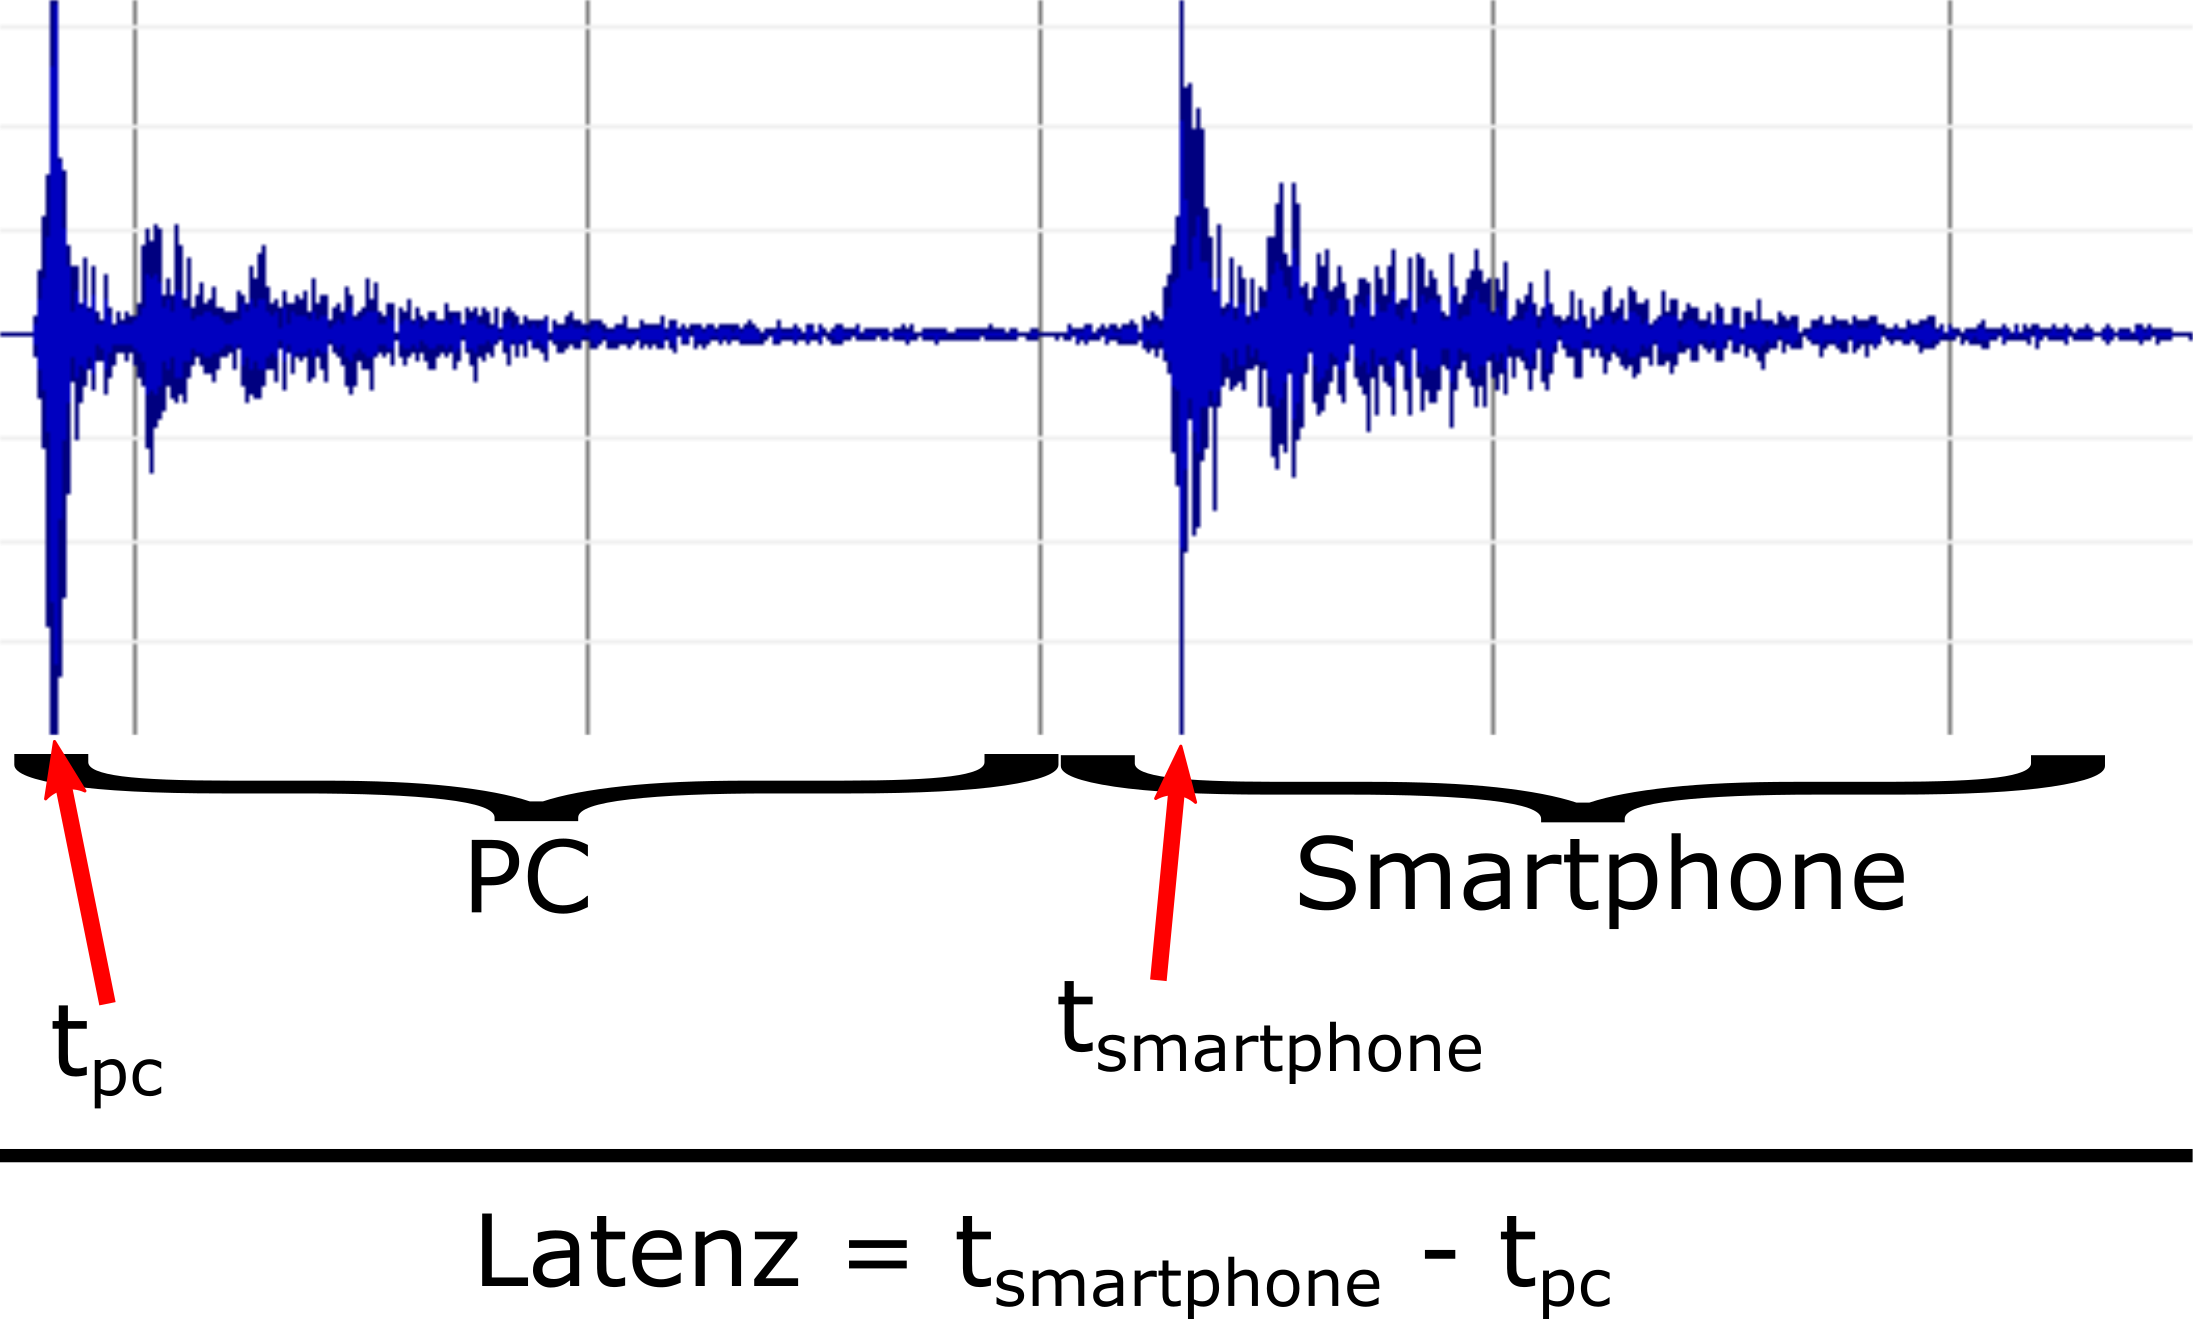
\includegraphics[width=0.7\textwidth]{img/spektrogramm.png}
		\caption{Bestimmung der Latenz anhand des Spektrogramms der Mikrofonaufnahme}
		\label{fig:spektrogramm}
	\end{center}
\end{figure}

Es wurden 30 Latenzmessungen pro Anwendung pro Smartphone aus den Leistungsklassen LOW (Samsung Galaxy S3 neo), MID (Samsung Galaxy S5) und HIGH (OnePlus 2) durchgeführt. Verwendet wurde ein PC mit Intel i7-3770k Prozessor. Die Qualität der Drahtlosübertragung kann die gemessene Latenz erheblich beeinflussen. Um den Einfluss der Übertragungsqualität einzuschränken, wurde für alle Messungen auf eine WiFi-Direct-Verbindung zurückgegriffen. Mithilfe der Anwendung Wifi Analyzer wurde zudem die Chance verringert, dass es während des Testens zu durch Interferenz verursachte Probleme kommt. Es wurde darauf geachtet, dass Audioqualität (48 kHz Stereo) und Puffergrößen bei allen Anwendungen gleich konfiguriert sind.

\section{Resultate}
Die in Abbildung \ref{boxplots} dargestellten Boxplots zeigen die Ergebnisse der insgesamt 9 Testreihen aufgeteilt auf die drei Leistungsklassen (LOW, MID, HIGH).


\begin{figure}[H]
\begin{subfigure}[b]{0.5\textwidth}
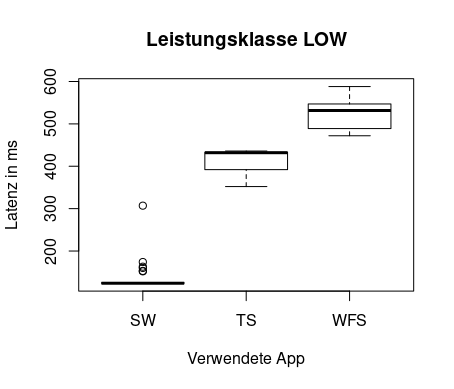
\includegraphics[width=\textwidth]{img/boxplotlow.png}
\end{subfigure}
\begin{subfigure}[b]{0.5\textwidth}
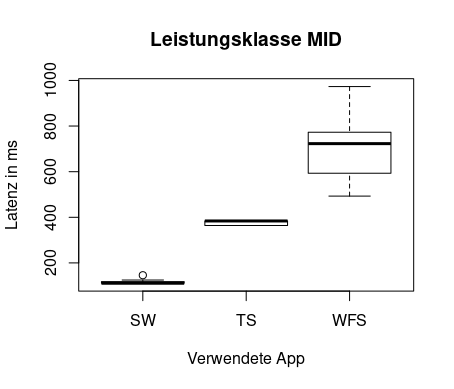
\includegraphics[width=\textwidth]{img/boxplotmid.png}
\end{subfigure}
\begin{subfigure}[b]{0.5\textwidth}
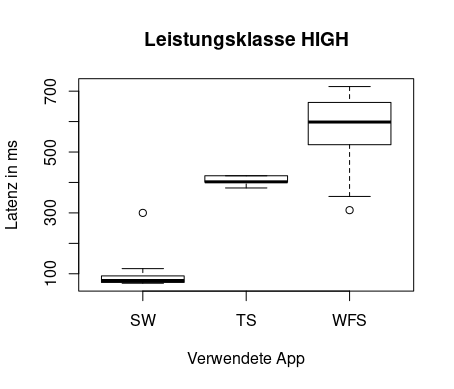
\includegraphics[width=\textwidth]{img/boxplothigh.png}
\end{subfigure}
\caption{Testergebnisse der insgesamt neun Testreihen}
\label{boxplots}
\end{figure}

Nach bloßem Betrachten der Ergebnisse lässt sich die Tendenz verzeichnen, dass bei allen Leistungsklassen SW die geringste Latenz aufweist. Die anschließende statistische Auswertung soll also folgende Hypothesen bestätigen:

\begin{itemize}
\item SW weißt eine geringere Latenz auf als TS.
\item SW weißt eine geringere Latenz auf als WFS.
\end{itemize}

Die Ergebnisse der einzelnen Testreihen wurden dem Shapiro-Wilk Test unterzogen, um auf Normalverteilung zu überprüfen. Nur die Datenreihe der Leistungsklasse LOW und der App WFS verzeichnete dabei einen p-Wert über dem Signifikanzniveau von 0.05 mit einem Wert von 0.06187, wodurch es sich wahrscheinlich um eine Normalverteilung handelt. Bei allen anderen Datenreihen ist anzunehmen, dass diese nicht auf einer Normalverteilung basieren.

In den meisten Datensätzen konnten wir keine Normalverteilung statistisch signifikant feststellen, allerdings sind in jeder Datenreihe 30 Ergebnisse enthalten. Dadurch ist es möglich, pro Geräteklasse einen T-Test zur Überprüfung der Hypothesen durchzuführen. Dabei ist zu beachten, dass der Datensatz von SW jeweils zweimal verwendet wird. Um das Problem des multiplen Testens zu umgehen, wird die Bonferoni-Korrektur angewandt. Dadurch wird das Signifikanzniveau halbiert und somit auf 0.025 gesetzt. Es werden pro Leistungsklasse zwei einseitige T-Tests durchgeführt, welche die Latenzen von SW mit TS und von SW mit WFS vergleichen.

\begin{table}[h]

\begin{tabular}{l|p{2cm}|p{2cm}|p{2cm}}
& LOW & MID & HIGH \\
\hline
SW/TS & t = -35.542; \newline df = 52.287; \newline p-value $< 2.2e-16$ & t = -116.18 \newline df = 51.875; \newline p-value $< 2.2e-16$ & t = -40.896 \newline df = 35.239; \newline p-value $< 2.2e-16$\\
\hline
SW/WFS & t = -44.652; \newline df = 57.64; \newline p-value $< 2.2e-16$ & t = -24.684; \newline df = 29.182; \newline p-value $< 2.2e-16$ & t = -24.806; \newline df = 38.176; \newline p-value $< 2.2e-16$ \\

\end{tabular}
\caption{Ergebnisse der T-Tests}
\end{table}

In allen T-Tests wird das Signifikanzniveau von 0.025 vom p-Wert klar unterschritten. Daraus folgt, dass die vorher aufgestellten Hypothesen akzeptiert werden können. Folgende 95\% Konfidenzintervalle wurden durch die T-Tests berechnet:

\begin{table}[h]

\begin{tabular}{l|p{2cm}|p{2cm}|p{2cm}}
& LOW & MID & HIGH \\
\hline
SW/TS & -Inf -0.2663635 & -Inf -0.2571063 & -Inf -0.3052234 \\
\hline
SW/WFS & -Inf -0.3753667 & -Inf -0.5284751 & -Inf -0.4623933 \\

\end{tabular}
\caption{95\% - Konfidenzintervalle der T-Tests}
\end{table}

Es kann abgelesen werden, dass in 95\% der Fälle die Latenz von SW je nach Leistungsklasse und zu vergleichender App zwischen rund 257ms und 528ms geringer ausfällt.

\section{Gefahren für die Validität \label{threats}}
Die größte Gefahr für die interne Validität stellt die Qualität der Drahtlosübertragung dar. Eine schlechte Verbindungsqualität kann eine höhere Latenz verursachen. Mithilfe der Anwendung WiFi Analyzer wurde über den gesamten Testzeitraum sichergestellt, dass keine anderen WiFi-Sender wesentlich aktiv sind. Jedoch konnte damit nicht sichergestellt werden, dass Sender, die eine andere Drahtlosübertragungstechnik wie 4g oder Bluetooth verwenden, zu einer Verschlechterung der Verbindungsqualität beitragen. Weiter ist die interne Validität des Experiments dadurch gefährdet, dass die Zeitwerte vom Spektrogramm von unterschiedlichen Personen anders abgelesen werden könnten. Um die Objektivität des Messvorgangs zu erhöhen, wurden alle Latenzwerte von drei Personen unabhängig abgelesen. Die maximale Abweichung zwischen den Messergebnissen unterschiedlicher Personen betrug lediglich eine Millisekunden. Durch die Wiederholung der Tests mit Smartphones unterschiedlicher Leistungsklassen wurde versucht, das Ergebnis auf eine größere Bandbreite von Smartphones verallgemeinerbar zu machen. Um die externe Validität zu erhöhen, ist es jedoch sinnvoll mit einer größeren Anzahl verschiedener Smartphones zu testen.

\section{Fazit}
Als klarer Sieger des Tests geht die App SoundWire hervor, da diese die geringste Latenz in allen Leistungsklassen aufweisen konnte. Wie auch schon in Kapitel \ref{threats} aufgezeigt, spielt die Qualität der WiFi-Verbindung eine entscheidende Rolle auf die Verzögerungszeit bei der drahtlosen Tonübertragung. In einem realen Umfeld, bei dem die Apps als Ersatz für Kabellose Kopfhörer zum Einsatz kommen sollen, muss klar nach Andwendungszweck unterschieden werden. Wird die Beschriebene Vorgehensweise beispielsweise zur Übertragung von Musik genutzt, stellt die Latenz keine Probleme dar. Die besten Latenzwerte die in unseren Tests gemessen wurden bewegten sich im Bereich knapp unter 100ms. Für Anwendungen im Filmbereich ist diese Latenz noch etwas zu groß. Eine Verzögerung von Ton- zur Videospur in dieser Größenordnung kann immer noch als störend empfunden werden. Es bleibt abzuwarten, ob in Zukunft Apps entwickelt werden, die diese Übertragungstechnik mit einer geringeren Latenz bewerkstelligen können. Außerdem ist es möglich, dass durch bessere WLAN-Technik eine Übertragung mit geringeren Verzögerungszeiten durchgeführt werden kann.


% An example of a floating figure using the graphicx package.
% Note that \label must occur AFTER (or within) \caption.
% For figures, \caption should occur after the \includegraphics.
% Note that IEEEtran v1.7 and later has special internal code that
% is designed to preserve the operation of \label within \caption
% even when the captionsoff option is in effect. However, because
% of issues like this, it may be the safest practice to put all your
% \label just after \caption rather than within \caption{}.
%
% Reminder: the "draftcls" or "draftclsnofoot", not "draft", class
% option should be used if it is desired that the figures are to be
% displayed while in draft mode.
%
%\begin{figure}[!t]
%\centering
%\includegraphics[width=2.5in]{myfigure}
% where an .eps filename suffix will be assumed under latex, 
% and a .pdf suffix will be assumed for pdflatex; or what has been declared
% via \DeclareGraphicsExtensions.
%\caption{Simulation results for the network.}
%\label{fig_sim}
%\end{figure}

% Note that the IEEE typically puts floats only at the top, even when this
% results in a large percentage of a column being occupied by floats.


% An example of a double column floating figure using two subfigures.
% (The subfig.sty package must be loaded for this to work.)
% The subfigure \label commands are set within each subfloat command,
% and the \label for the overall figure must come after \caption.
% \hfil is used as a separator to get equal spacing.
% Watch out that the combined width of all the subfigures on a 
% line do not exceed the text width or a line break will occur.
%
%\begin{figure*}[!t]
%\centering
%\subfloat[Case I]{\includegraphics[width=2.5in]{box}%
%\label{fig_first_case}}
%\hfil
%\subfloat[Case II]{\includegraphics[width=2.5in]{box}%
%\label{fig_second_case}}
%\caption{Simulation results for the network.}
%\label{fig_sim}
%\end{figure*}
%
% Note that often IEEE papers with subfigures do not employ subfigure
% captions (using the optional argument to \subfloat[]), but instead will
% reference/describe all of them (a), (b), etc., within the main caption.
% Be aware that for subfig.sty to generate the (a), (b), etc., subfigure
% labels, the optional argument to \subfloat must be present. If a
% subcaption is not desired, just leave its contents blank,
% e.g., \subfloat[].


% An example of a floating table. Note that, for IEEE style tables, the
% \caption command should come BEFORE the table and, given that table
% captions serve much like titles, are usually capitalized except for words
% such as a, an, and, as, at, but, by, for, in, nor, of, on, or, the, to
% and up, which are usually not capitalized unless they are the first or
% last word of the caption. Table text will default to \footnotesize as
% the IEEE normally uses this smaller font for tables.
% The \label must come after \caption as always.
%
%\begin{table}[!t]
%% increase table row spacing, adjust to taste
%\renewcommand{\arraystretch}{1.3}
% if using array.sty, it might be a good idea to tweak the value of
% \extrarowheight as needed to properly center the text within the cells
%\caption{An Example of a Table}
%\label{table_example}
%\centering
%% Some packages, such as MDW tools, offer better commands for making tables
%% than the plain LaTeX2e tabular which is used here.
%\begin{tabular}{|c||c|}
%\hline
%One & Two\\
%\hline
%Three & Four\\
%\hline
%\end{tabular}
%\end{table}


% Note that the IEEE does not put floats in the very first column
% - or typically anywhere on the first page for that matter. Also,
% in-text middle ("here") positioning is typically not used, but it
% is allowed and encouraged for Computer Society conferences (but
% not Computer Society journals). Most IEEE journals/conferences use
% top floats exclusively. 
% Note that, LaTeX2e, unlike IEEE journals/conferences, places
% footnotes above bottom floats. This can be corrected via the
% \fnbelowfloat command of the stfloats package.





% conference papers do not normally have an appendix


% use section* for acknowledgment






% trigger a \newpage just before the given reference
% number - used to balance the columns on the last page
% adjust value as needed - may need to be readjusted if
% the document is modified later
%\IEEEtriggeratref{8}
% The "triggered" command can be changed if desired:
%\IEEEtriggercmd{\enlargethispage{-5in}}

% references section

% can use a bibliography generated by BibTeX as a .bbl file
% BibTeX documentation can be easily obtained at:
% http://mirror.ctan.org/biblio/bibtex/contrib/doc/
% The IEEEtran BibTeX style support page is at:
% http://www.michaelshell.org/tex/ieeetran/bibtex/
%\bibliographystyle{IEEEtran}
% argument is your BibTeX string definitions and bibliography database(s)
%\bibliography{IEEEabrv,../bib/paper}
%
% <OR> manually copy in the resultant .bbl file
% set second argument of \begin to the number of references
% (used to reserve space for the reference number labels box)
%\begin{thebibliography}{1}

%\bibitem{IEEEhowto:kopka}
%H.~Kopka and P.~W. Daly, \emph{A Guide to \LaTeX}, 3rd~ed.\hskip 1em plus
%  0.5em minus 0.4em\relax Harlow, England: Addison-Wesley, 1999.

%\end{thebibliography}




% that's all folks
\end{document}


